% COSC418 Final Presentation
% Regan Gunther and Henry Jenkins - 2011

%\documentclass[handout]{beamer}
\documentclass{beamer}

\usetheme[secheader]{Boadilla}
\usecolortheme{seahorse}
\usepackage[latin1]{inputenc}
\usepackage{mathtools}
\usepackage{listings}
\usepackage{verbatim}
\usepackage{graphics}


\title{COSC418 Project:\\Load balancing in a CTP based network}
\author{Henry Jenkins and Regan Gunther}
\date{September 30, 2011}
\institute[2011]{Department of Computer and Electrical Engineering,\\
    University of Canterbury, \\ Christchurch, \\ New Zealand}

\begin{document}

\frame{\titlepage}

\section[Outline]{}
\frame{\tableofcontents}

\section{Design}
\subsection{Overview}

\begin{frame}[fragile]
  \frametitle{UnicastNameFreeRouting}
  
    \begin{itemize}
      \item We took the original UnicastNameFreeRouting interface
            and turned this into UnicastNameFreeLoadBalRouting by adding extra
            load balancing features.
    \end{itemize}

  \footnotesize{
    \begin{block}{Code Implementation}
      \begin{verbatim}
interface UnicastNameFreeLoadBalRouting {

  command am_addr_t nextHop();
  command bool hasRoute();
  //Triggers a packet notification
  command void packetSent();
  
  event void routeFound();
  event void noRoute();
}
      \end{verbatim}
    \end{block}
  }
  \begin{itemize}
    \item Interface provided by CtpRoutingEngine and used by
    MultiHopOscilloscope
  \end{itemize}
\end{frame}


\section{Implementation}
\subsection{Code}

\begin{frame}[fragile]
  \frametitle{Our Design}
  \begin{itemize}
    \item $p^* = \text{arg min}  p \in \{\ \text{direct neighbours} \}\
                 [\alpha  \cdot (ETX_{s,p} + ETX_p) + \beta \cdot L_p^s]$

    \item Our design is to keep $L_p^s$ locally
  \end{itemize} 
   
  \footnotesize{
  \begin{block}{Code Implementation}
    \begin{verbatim}
// ETX for load balancing                                                                                                                                                              
uint16_t loadEtx;

//Complete Equation:
beaconMsg->etx = routeInfo.etx + 
call LinkEstimator.getLinkQuality(routeInfo.parent) 
+ (loadEtx/LOAD_EFFECT_THRESHOLD);
    \end{verbatim}
  \end{block}
}
\end{frame}

\begin{frame}[fragile]
  \frametitle{$t_p^s$}
  \footnotesize{
    \begin{block}{Code Implementation}
      \begin{verbatim}
/* 
 * Timer for the load balancing algorithm
 */
event void LoadTimer.fired() {
  //First decrement loadEtx to ensure decay
  if (loadEtx > 0) {
    loadEtx--;
  }
  //If there is a large change in loadEtx tell nabours
  if (radioOn && running) {
    if (loadEtx > oldLoadEtx + 10 || 
        (oldLoadEtx > 10 && loadEtx < oldLoadEtx - 10)) {
      post sendBeaconTask();
    }
  }
}
      \end{verbatim}
    \end{block}
  }
\end{frame}

\begin{frame}[fragile]
  \frametitle{$n_p^s$}
  \footnotesize{
    \begin{block}{Code Implementation}
      \begin{verbatim}
/*
 * This is to be called when ever a packet is sent via the radio.
 */
command void Routing.packetSent() {
  loadEtx++;
  printf("P\n");
  //printf("Load ETX Incremented. It is now: %d\n",loadEtx);
  //printfflush();
}
      \end{verbatim}
    \end{block}
  }
\end{frame}


\begin{frame}[fragile]
  \frametitle{Parameter Definitions}
  In TreeRouting.h:
  \footnotesize{
    \begin{block}{Code Implementation}
      \begin{verbatim}
enum {
    ...

    // Load balancing timer
    LOAD_INTERVAL = 100,        

    //Number of packets per rollover
    LOAD_EFFECT_THRESHOLD = 1, 

    ...
}; 
      \end{verbatim}
    \end{block}

    \begin{itemize}
      \item This allowed for easy access of values during the testing stage
    \end{itemize}
  }
\end{frame}



\begin{frame}[fragile]
  \frametitle{Figure}
   % \includegraphics[width=\textwidth]{Demo_s1}
  \footnotesize{
    \begin{block}{Figure}
        \includegraphics[width=\textwidth]{Images/Demo_s1}
    \end{block}

    \begin{itemize}
      \item This allowed for easy access of values during the testing stage
    \end{itemize}
  }
\end{frame}







\subsection{Drawbacks}

\begin{frame}[fragile]
  \frametitle{Drawbacks}
    What if $ETX_p + ETX_{p,s} + L_p^s$ (i.e. $ETX_s$) increases to be $\geq 2^{16}$?
  \begin{itemize}
    \item Bad things\ldots
    \item This is managed by including the $t_p^s$ in the loading parameter
    $L_p^s$
    \item (Remember $L_p^s = n_p^s - t_p^s$ )
    \item Periodic timer.
  \end{itemize}

\end{frame}  



\begin{frame}
  \frametitle{Drawbacks}
    ETX changing with each packet transmission causes routing updates all the
    time. All these updates would be inefficient.
  \begin{itemize}
    \item A solution to this is to only update routes when ETX changes by a given
    threshold
    \end{itemize}
\end{frame}  


\begin{frame}
  \frametitle{Drawbacks}
    Exponential ETX growth of a node
  \begin{itemize}
    \item In a path of 5 nodes to the root, $L_p^s$ increases with every packet.
    The more hops to the root, the more pronounced this effect
  \end{itemize}
\end{frame}  


\section{Results \& Conclusions}
\subsection{Testing}
%wank on about using Mviz

\subsection{Conclusions}

\begin{frame}
  \frametitle{Conclusion}
  \begin{itemize}
    \item No results as yet
    \item Currently implementing and testing code
  \end{itemize}
\end{frame}  


\end{document}
